\documentclass{article}
    \usepackage[fontset = windowsnew]{ctex}
        \CTEXoptions[today=old]
        \ctexset{figurename=Figure}
    \usepackage{geometry}
        \geometry{left=2.54cm,right=2.54cm,top=2.54cm,bottom=2.54cm}
    \usepackage{amsmath}
    \usepackage{amsfonts}
    \usepackage{siunitx}
    \usepackage{booktabs}
    \usepackage{longtable}
    \usepackage{graphicx}
    \usepackage{subfig}
    \usepackage{float}
    \usepackage{fancyvrb}
    \renewcommand{\labelenumi}{\alph{enumi}.} % Make numbering in the enumerate environment by letter rather than number

    \title{\textbf{数字逻辑与处理器基础实验} \\ [2ex] \begin{large} \emph{32位MIPS处理器设计实验报告} \end{large} }
    \author{王晗 \\ (2013011076)}
    \date{\today}

\begin{document}
    \maketitle

    \begin{table}[htb]
        \centering
        \begin{tabular}{lr}
            Date Performed: & July 15, 2015 \\
            Partners:   & 耿天毅(2012011119) \\
                        & 陈志杰 \fbox{\begin{small}\emph{~~withdrawn~~}\end{small}} \\
        \end{tabular}
    \end{table}

    \section{实验目的}
        熟悉现代处理器的基本工作原理;掌握单周期和流水线处理器的设计方法。

    \section{设计方案}
        \subsection{总体结构}
            由于这次实验涉及的功能较多,我们将完整的CPU分成多个模块。指令存储器、寄存器堆、控制器、ALU控制器、ALU、数据存储器、UART等功能单元均在单独的Module中实现。其中指令存储器、寄存器堆、控制器、ALU控制器、ALU等单元在Single Cycle Core中实例化,作为单周期处理器的核心;数据存储器、UART和定时器、LED、七段数码管、开关在Peripheral中实现,作为处理器的外设。处理器核心和外设在顶层模块中实例化,互相通信。
            
            单周期CPU模块的结构关系如下图所示:
            \begin{figure}[H]
                    \centering
                    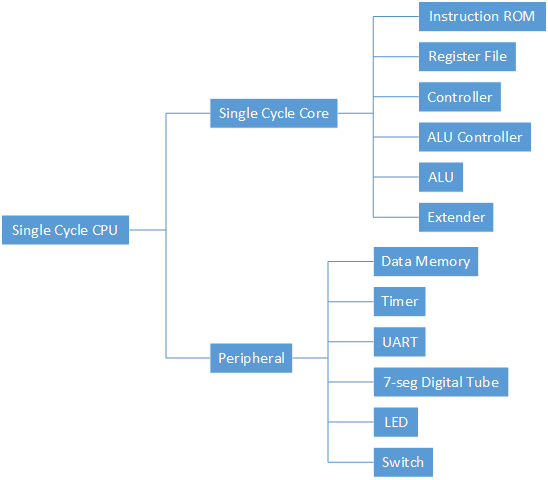
\includegraphics[width=0.62\textwidth]{images/singlecycle.png}
                    \caption{\label{fig:singlecycle}单周期处理器结构}
                \end{figure}
            
            对于流水线CPU,我们还在Pipeline Core中加入了流水线寄存器、冒险检测单元、数据转发单元:
            \begin{figure}[H]
                    \centering
                    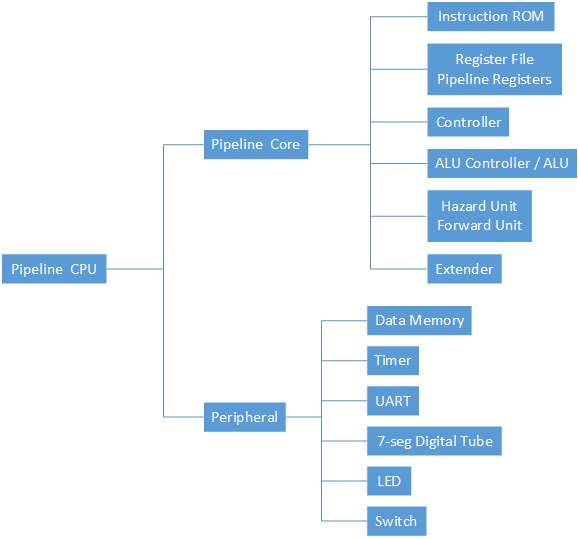
\includegraphics[width=0.62\textwidth]{images/pipeline.png}
                    \caption{\label{fig:pipeline}流水线处理器结构}
                \end{figure}
            
        \subsection{ALU \protect\footnote{原作者:陈志杰;修改:王晗}}
            ALU模块的结构如图所示,输入两个操作数A、B和控制信号ALUFun、Signed,在ARITH子模块中做加减法运算,CMP子模块根据ARITH模块的输出进行比较判断,LOGIC和SHIFT模块分别进行逻辑运算和移位运算,ALUFun的最高两位用于控制多路选择器的输出。
            \begin{figure}[H]
                    \centering
                    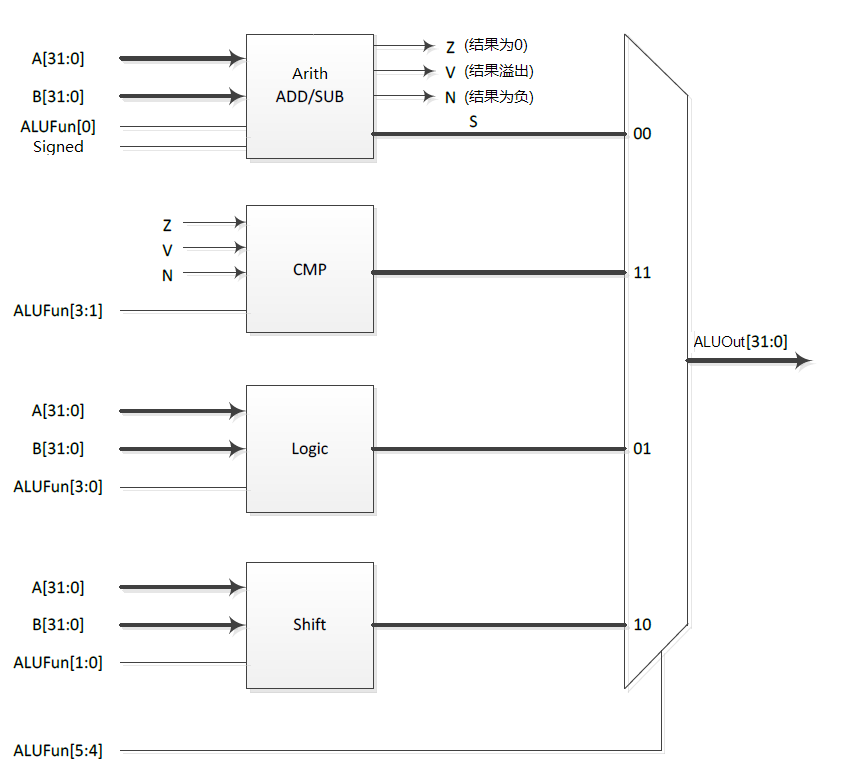
\includegraphics[width=0.62\textwidth]{images/ALU.png}
                    \caption{\label{fig:ALU}流水线处理器结构}
                \end{figure}
            
            \paragraph*{ARITH模块}
            ARITH模块中包括减法和加法两个模块,加法模块直接通过+号运算,减法模块先对第二个操作数取补码,再调用加法模块做加法运算。Overflow和Negative信号的产生是ALU中的难点:
            \begin{figure}[H]
                \centering
                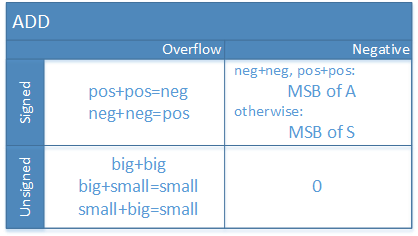
\includegraphics[width=0.5\textwidth]{images/add_v_n.png}
                \caption{\label{fig:add_v_n}ADD中的Overflow和Negative}
            \end{figure}
            其中pos为正数,neg为负数,big为MSB=1的无符号数,small为MSB=0的无符号数。
            
            \begin{figure}[H]
                \centering
                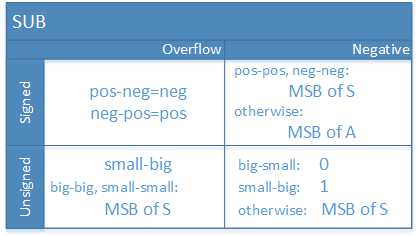
\includegraphics[width=0.5\textwidth]{images/sub_v_n.png}
                \caption{\label{fig:sub_v_n}SUB中的Overflow和Negative}
            \end{figure}
            图中的缩写含义同上。
            
            \paragraph*{CMP模块}
            CMP模块直接根据ARITH模块产生的Zero, Overflow, Negative进行关系判断。
            
            \paragraph*{LOGIC模块}
            LOGIC模块直接根据ALUFun[3:0]指定的逻辑运算进行运算。
            
            \paragraph*{SHIFT模块}
            将移位操作拆分为16位移位、8位移位、4位移位、2位移位、1位移位,分别用Shamt的每一个bit位控制,组合产生最后的运算结果。
            
        \subsection{寄存器堆、指令存储器、数据存储器和外设 \protect\footnote{作者:王晗}}
            \paragraph*{寄存器堆}
                直接采用reg [31:0] RF\_DATA[31:1]实现,注意RF\_DATA[0]不存在,读取时直接返回0。
            \paragraph*{指令存储器}
                将机器码以十六进制文本的形式存放在.rom文件中,使用\$readmemh系统任务初始化一个大小为256words的只读存储器。
            \paragraph*{数据存储器}
                由于数据存储器容量设计为256words,因此寻址时只根据address[9:2]寻址。 \\ 
                另外,0x40000000开始的地址用于外设编址,因此数据存储器不对0x40000000开始的地址进行读写操作。
            \paragraph*{其他外设}   
                定时器、LED、Switch参考老师提供的样例代码直接在Peripheral.v中实现,UART使用春季学期第四次实验的UART发送和接收模块,将发送模块中Tx\_Status的定义取反,即1表示发送端忙碌。UART的控制同样在Peripheral.v中实现,当0x40000018写入要发送的数据时,串口控制器自动产生一个发送使能信号。
                
        \subsection{控制器和ALU控制器 \protect\footnote{作者:王晗}}
            控制单元采用两级控制的实现方法,在主控制器中根据OpCode和Funct产生PCSrc、RegWrite、RegDst、MemRead、MemWrite、MemToReg、ALUSrc1、ALUSrc2、ExtOp、LuOp、ALUOp等控制信号,其中ALUOp 经过ALU控制器进一步解码生成ALUFunc、Signed信号,控制ALU的运算,其余信号控制数据通路中的多路选择器。控制器还产生了UndefinedInst信号,用于识别未定义指令的异常。
           
            在单周期CPU中,PCSrc信号位宽为2,分别指示从PC+4、Branch Target、Jump Target、Jump Register取出下一个指令地址,当发生中断或异常时,由Single-Cycle Core直接跳转至中断或异常服务程序入口。在流水线CPU中,为了方便流水线寄存器操作,将PCSrc信号位宽扩展至3,当发生中断或异常,PCSrc变为100或101,指示中断或异常服务程序入口。
            
        \subsection{单周期数据通路 \protect\footnote{作者:王晗}}
            \begin{figure}[H]
                \centering
                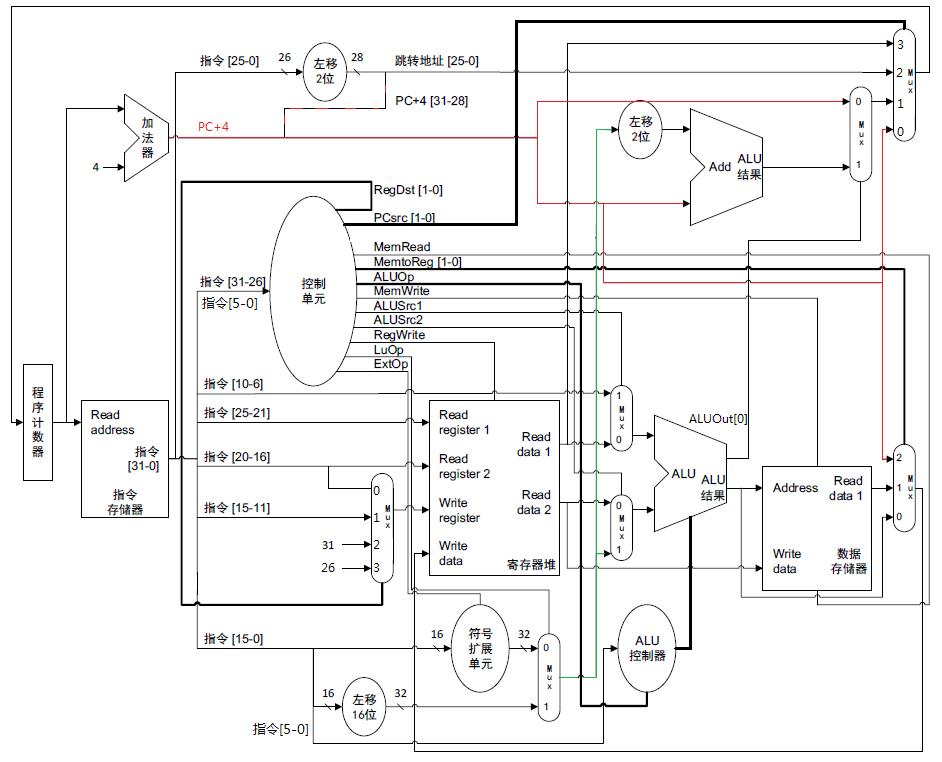
\includegraphics[width=0.95\textwidth]{images/singlecycle_datapath.png}
                \caption{\label{fig:singlecycle_datapath}单周期数据通路}
            \end{figure}
            
        \subsection{流水线数据通路 \protect\footnote{作者:王晗}}

        \subsection{汇编代码 \protect\footnote{作者:耿天毅}}
        
        \subsection{汇编器 \protect\footnote{作者:耿天毅}}

    \section{关键代码及文件清单}

    \section{仿真结果及分析}

    \section{硬件调试情况}
        硬件调试情况

    \section{心得体会}

        \begin{enumerate}
            \begin{item}
                我没有
            \end{item}
            \begin{item}
                心得
            \end{item}
            \begin{item}
                体会
            \end{item}
        \end{enumerate}

\end{document}
